\documentclass{npj-article}

\title{Supplementary Information: Martian Crustal Magnetic Field Heterogeneity and Implications for Biological Systems at Candidate Landing Sites}

\author{%
  \textbf{Richard Barker}\textsuperscript{1,*},
  \textbf{Adriana Kaley Sanchez}\textsuperscript{1},
  \textbf{Manisha Dagar}\textsuperscript{1},
  \textbf{Katrina Boland}\textsuperscript{1},
  \textbf{Cau\^{e} Sciascia Borlina}\textsuperscript{2},
  \textbf{D.~Marshall Porterfield}\textsuperscript{1}
  \vspace{2mm}\\
  \textsuperscript{1}\footnotesize Department of Agricultural and Biological Engineering, Purdue University, West Lafayette, IN 47907, USA\\
  \textsuperscript{2}\footnotesize Department of Earth, Atmospheric, and Planetary Sciences, Purdue University, West Lafayette, IN 47907, USA\\
  \textsuperscript{*}\footnotesize Corresponding author: \href{mailto:rbarker2@purdue.edu}{rbarker2@purdue.edu}
}

\begin{document}
\makefrontmatter

\section*{Extended Methods}

\subsection*{Spherical Harmonic Model and Vector Field Processing}
Martian crustal magnetic field components ($B_r, B_\theta, B_\phi$) were computed using the spherical harmonic potential model developed by \citet{Langlais2019}, derived from joint inversions of nightside orbital data from Mars Global Surveyor (MGS) at \SI{400}{\kilo\meter} circular mapping altitude and MAVEN elliptical periapsis tracks down to $\sim\SI{130}{\kilo\meter}$.

\subsection*{Ground-Truth Comparison with InSight Magnetometer}
Direct in situ ground-truth validation was integrated using calibrated surface magnetometer measurements from the InSight Fluxgate (IFG) Magnetometer in Elysium Planitia ($\SI{4.50}{\degree}\text{N}$, $\SI{135.62}{\degree}\text{E}$). The InSight surface measurement of $\sim\SI{2013}{\nano\tesla}$ \citep{Johnson2020} confirms that shallow, localized crustal sources in the subsurface can produce ground-level fields an order of magnitude higher than orbital baseline projections.

\section*{Supplementary Figures}

\begin{figure*}[h]
\centering
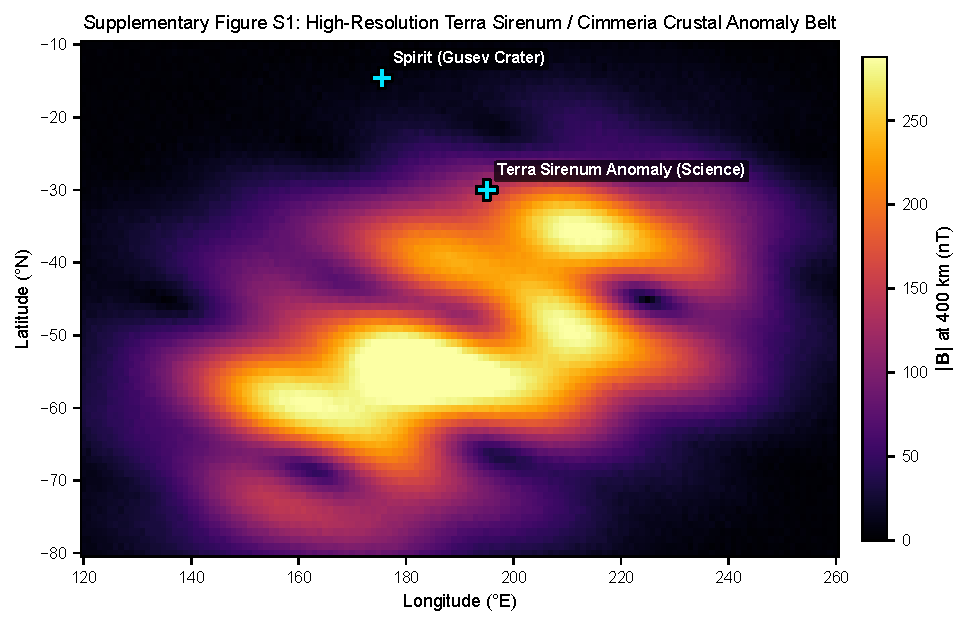
\includegraphics[width=0.85\textwidth]{../figures/fig_S1_terra_sirenum_detail.pdf}
\caption{\textbf{Supplementary Figure S1 \textbar\ High-resolution regional magnetic field map of the Terra Sirenum / Terra Cimmeria crustal anomaly belt.} Map spans $\SI{120}{\degree}\text{E}$ to $\SI{260}{\degree}\text{E}$ longitude and $\SI{10}{\degree}\text{S}$ to $\SI{80}{\degree}\text{S}$ latitude at \SI{400}{\kilo\meter} altitude, highlighting coherent crustal magnetic lineations and candidate scientific outpost coordinates.}
\label{fig:S1_terra_sirenum_detail}
\end{figure*}

\begin{figure*}[h]
\centering
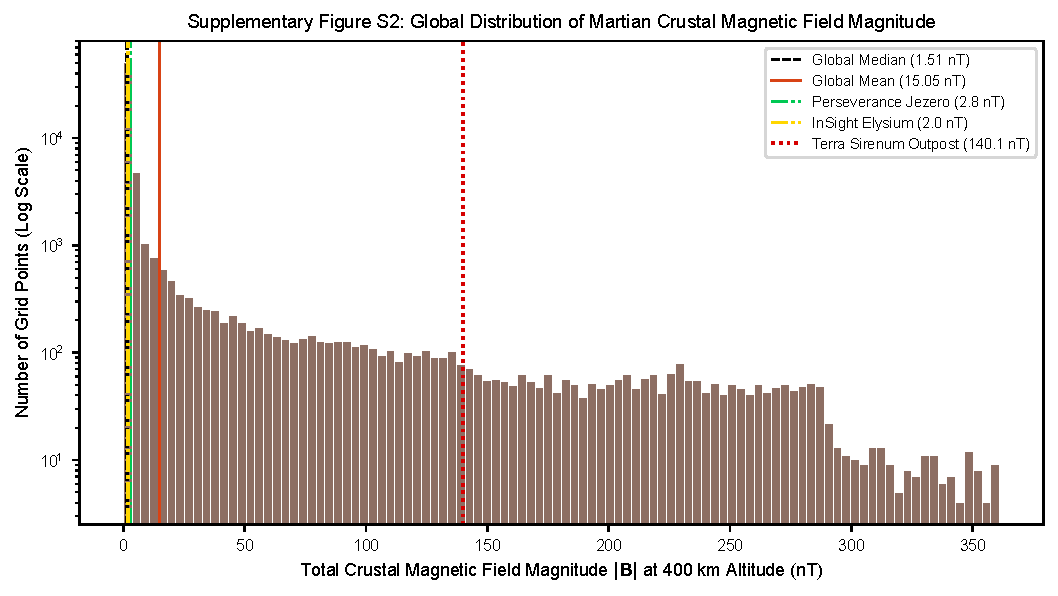
\includegraphics[width=0.85\textwidth]{../figures/fig_S2_mars_field_histogram.pdf}
\caption{\textbf{Supplementary Figure S2 \textbar\ Global frequency distribution of Martian crustal magnetic field magnitude.} Histogram displaying $|\mathbf{B}|$ at \SI{400}{\kilo\meter} altitude across 65,160 global grid points, with global median (\SI{1.51}{\nano\tesla}), global mean (\SI{15.05}{\nano\tesla}), Perseverance Jezero site (\SI{2.75}{\nano\tesla}), InSight Elysium site (\SI{1.99}{\nano\tesla}), and Terra Sirenum outpost (\SI{140.07}{\nano\tesla}) highlighted.}
\label{fig:S2_mars_field_histogram}
\end{figure*}

\section*{Data and Code Availability}
The full machine-readable landing site database, processed global grids, figure generation scripts, and interactive 3D WebGL globe source code are available in the public GitHub repository (\url{https://github.com/dr-richard-barker/mars-magnetic-biology}) and archived under DOI: \href{https://doi.org/10.5281/zenodo.XXXXXXX}{10.5281/zenodo.XXXXXXX}.

\renewcommand{\bibnumfmt}[1]{#1.}
\bibliographystyle{unsrtnat}
\bibliography{references}

\end{document}
